% 2009 年上海卷文科第 16 题：底面为直角三角形、侧棱垂直于底面的三棱锥及其主视图四选项。
% 来源 PDF：普通高考/2009/2009上海文.pdf，SHA256 5212f16aacbac7b10c5df44f90ccd94ba0218c31c04bd0c4e9e0e8f0284ca5f3
% 原页：第 1 页（A3 三栏）第 2 栏下部，印刷页 555。
% 重绘依据：上方小图为三棱锥与坐标轴（z 向上、x 向前左、y 向右），底面直角边 3、4，
%   直角顶点处侧棱高 4；下方四选项为直角三角形轮廓：(A) 4×4、(B) 3×4、(C) 3×4
%   （直角在右上）、(D) 斜边 5、高 4；标注与直角记号按原图。
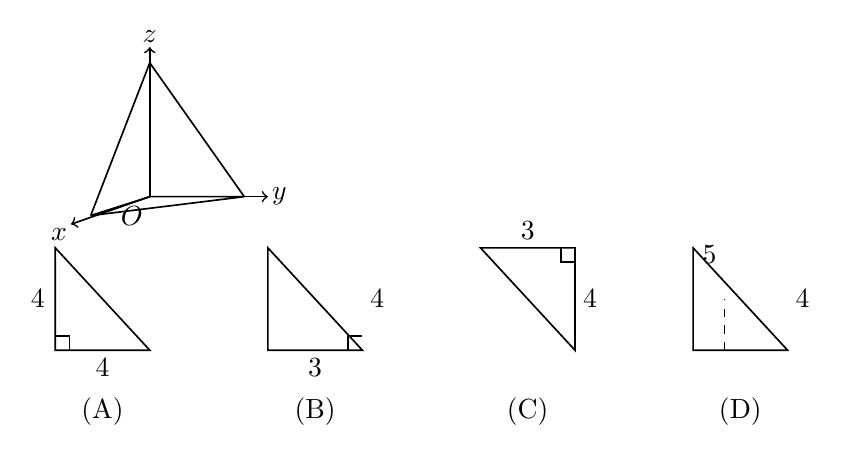
\begin{tikzpicture}[scale=1.0, semithick, every node/.style={inner sep=1.2pt}]
  % ---------- 上方立体示意 ----------
  \coordinate (O) at (1.2,0.5);
  \draw[->] (O) -- (0.2,0.15) node[anchor=north east] {$x$};
  \draw[->] (O) -- (2.7,0.5) node[anchor=west] {$y$};
  \draw[->] (O) -- (1.2,2.4) node[anchor=south] {$z$};
  \coordinate (P) at (1.2,2.2);
  \coordinate (X) at (0.45,0.26);
  \coordinate (Y) at (2.4,0.5);
  \draw (O) -- (X) -- (Y) -- cycle;
  \draw (P) -- (X);
  \draw (P) -- (Y);
  \draw (P) -- (O);
  \node[anchor=north east] at ([xshift=-1pt,yshift=-2pt]O) {$O$};
  % ---------- 四个选项 ----------
  \foreach \dx/\opt in {0/A, 2.7/B, 5.4/C, 8.1/D} {
    \node[anchor=north] at (\dx+0.6,-2.0) {(\opt)};
  }
  % (A) 4 x 4，直角在左下
  \draw (0,-0.15) -- (0,-1.45) -- (1.2,-1.45) -- cycle;
  \draw (0.18,-1.45) -- (0.18,-1.27) -- (0,-1.27);
  \node[anchor=east] at (-0.08,-0.8) {$4$};
  \node[anchor=north] at (0.6,-1.5) {$4$};
  % (B) 3 x 4，直角在右下
  \draw (2.7,-0.15) -- (2.7,-1.45) -- (3.9,-1.45) -- cycle;
  \draw (3.72,-1.45) -- (3.72,-1.27) -- (3.9,-1.27);
  \node[anchor=west] at (3.95,-0.8) {$4$};
  \node[anchor=north] at (3.3,-1.5) {$3$};
  % (C) 上边 3、右边 4，直角在右上
  \draw (5.4,-0.15) -- (6.6,-0.15) -- (6.6,-1.45) -- cycle;
  \draw (6.42,-0.15) -- (6.42,-0.33) -- (6.6,-0.33);
  \node[anchor=south] at (6.0,-0.1) {$3$};
  \node[anchor=west] at (6.65,-0.8) {$4$};
  % (D) 斜边 5、高 4，直角在右下
  \draw (8.1,-0.15) -- (8.1,-1.45) -- (9.3,-1.45) -- cycle;
  \draw[dashed] (8.5,-1.45) -- (8.5,-0.8);
  \node[anchor=south east] at (8.45,-0.4) {$5$};
  \node[anchor=west] at (9.35,-0.8) {$4$};
\end{tikzpicture}
